\chapter{Analyse et spécification des besoins}
\label{chap:analyse_besoins}

\section{Introduction}

L'analyse et la spécification des besoins constituent une étape fondamentale dans le cycle de vie du développement logiciel. Cette phase permet de définir précisément ce que le système doit faire (besoins fonctionnels) et comment il doit se comporter (besoins non fonctionnels), tout en identifiant les différents acteurs interagissant avec la plateforme. 

Ce chapitre expose les exigences du projet Alpha Store, une plateforme e-commerce multi-secteurs augmentée par l'intelligence artificielle. Nous y détaillerons l'identification des acteurs, la spécification détaillée des fonctionnalités ainsi que la modélisation UML des principaux cas d'utilisation.

\section{Spécification des besoins}

\subsection{Identification des acteurs}

Pour Alpha Store, nous avons identifié trois types d'acteurs principaux ayant des interactions distinctes avec le système :

\begin{itemize}[label=$\bullet$]
    \item \textbf{Visiteur (Internaute) :} Tout utilisateur non connecté qui accède à la plateforme pour consulter le catalogue (Mode et Tech), filtrer les produits et visualiser les détails sans pouvoir effectuer d'achat ou accéder aux fonctions personnalisées.
    \item \textbf{Client (Utilisateur connecté) :} Acteur principal qui, après authentification, peut gérer son panier, passer des commandes, soumettre des avis, gérer ses favoris et utiliser l'ensemble des modules d'intelligence artificielle (Configurateur PC, Mix \& Match, Smart Budget, Try-On).
    \item \textbf{Administrateur :} Responsable de la gestion opérationnelle de la plateforme via un tableau de bord dédié (gestion du stock, des catégories, des commandes et des utilisateurs).
\end{itemize}

\subsection{Besoins fonctionnels}

Les besoins fonctionnels décrivent les services offerts par la plateforme Alpha Store.

\begin{enumerate}
    \item \textbf{Gestion du catalogue et recherche :}
        \begin{itemize}[label=$\bullet$]
            \item Consultation des produits par secteurs (Mode Homme/Femme/Enfant et Technologie).
            \item Filtrage avancé par catégorie, prix, couleur et spécifications techniques.
            \item Système de recommandation intelligente basé sur les algorithmes BFS et DFS.
        \end{itemize}
    \item \textbf{Gestion du cycle d'achat :}
        \begin{itemize}[label=$\bullet$]
            \item Gestion du panier (ajout, modification de quantité, suppression).
            \item Processus de commande sécurisé avec récapitulatif.
            \item Suivi des commandes et historique d'achat via le tableau de bord client.
        \end{itemize}
    \item \textbf{Intelligence Artificielle et Assistance :}
        \begin{itemize}[label=$\bullet$]
            \item \textbf{PC Builder :} Configuration de PC avec vérification de compatibilité (CSP) et optimisation par Algorithme Génétique.
            \item \textbf{Mix \& Match :} Suggestion de tenues coordonnées basées sur des contraintes de style et de saison (CSP).
            \item \textbf{Smart Budget :} Optimisation des achats selon une enveloppe budgétaire (Algorithme Génétique).
            \item \textbf{Virtual Try-On :} Essayage virtuel de vêtements via l'IA IDM-VTON.
            \item \textbf{Chatbot Gemini :} Assistance conversationnelle en langage naturel pour le conseil produit.
        \end{itemize}
    \item \textbf{Engagement et Sécurité :}
        \begin{itemize}[label=$\bullet$]
            \item Authentification sécurisée avec vérification par code OTP.
            \item Système de gamification (Roue des prix) pour la fidélisation.
            \item Gestion du profil utilisateur et des listes de favoris.
        \end{itemize}
\end{enumerate}

\subsection{Besoins non fonctionnels}

\begin{itemize}[label=$\bullet$]
    \item \textbf{Ergonomie et UX :} L'interface doit être fluide, moderne et réactive, exploitant les animations GSAP pour une expérience premium.
    \item \textbf{Sécurité :} Protection des données utilisateurs via le hachage Bcrypt et sécurisation des échanges contre les failles courantes (SQLi, XSS).
    \item \textbf{Performance :} Temps de réponse optimal, notamment pour les calculs d'IA qui doivent être gérés de manière asynchrone ou via des microservices légers.
    \item \textbf{Disponibilité :} La plateforme doit être accessible 24/7 avec une gestion robuste des erreurs (page 404 personnalisée).
\end{itemize}

\section{Modélisation des besoins}

\subsection{Langage de Modélisation UML}

Pour modéliser les besoins de notre système, nous utilisons le langage UML (Unified Modeling Language), standard de l'industrie pour la visualisation, la spécification et la documentation des systèmes logiciels.

\begin{figure}[H]
    \centering
    
\includegraphics[scale=0.1]{chapitre2/figuresChap2/UML.png}
    \caption{Logo d'UML}
    \label{fig:uml_logo}
\end{figure}


\subsection{Diagrammes de cas d’utilisation}

\subsubsection{Diagramme de cas d'utilisation global}

Le diagramme global présente une vue d'ensemble des interactions entre les différents acteurs et les fonctionnalités majeures de la plateforme Alpha Store.

\clearpage
\begin{figure}[p]
    \centering
    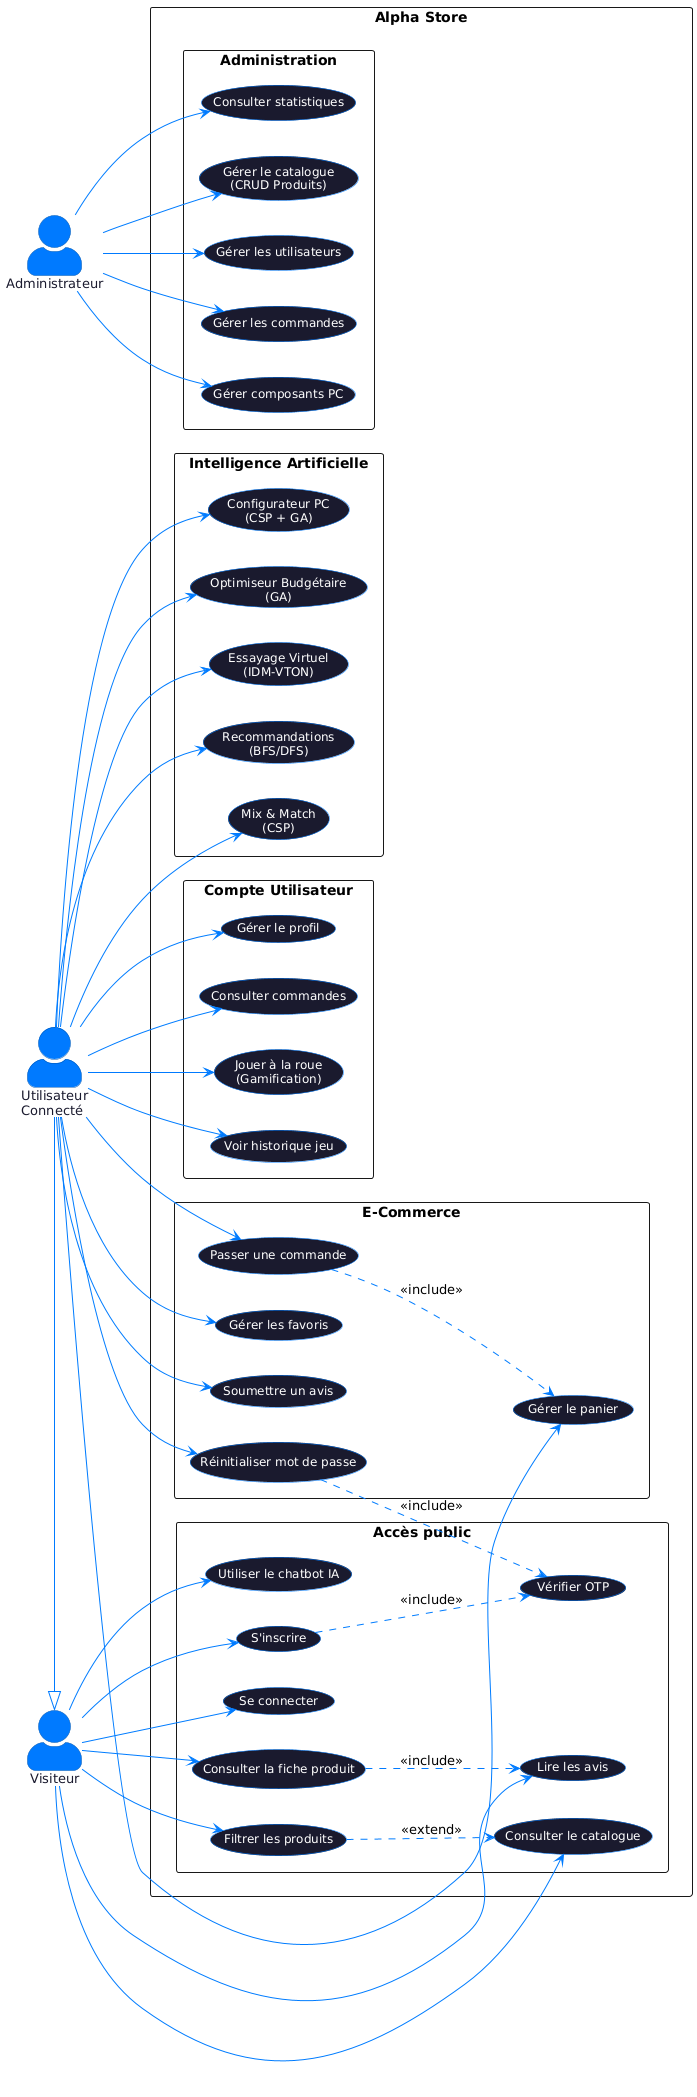
\includegraphics[height=0.82\textheight,keepaspectratio]{chapitre2/figuresChap2/usercase.png}
    \caption{Diagramme de cas d'utilisation global}
    \label{fig:uc_global}
\end{figure}
\clearpage

\subsubsection{Diagrammes détaillés par acteur}

Pour une meilleure lisibilité, nous détaillons ci-dessous les cas d'utilisation spécifiques à chaque type d'acteur.

\paragraph{Diagramme Visiteur :} 
Le visiteur peut principalement consulter le catalogue, rechercher des produits et visualiser les détails.
\begin{figure}[H]
    \centering
    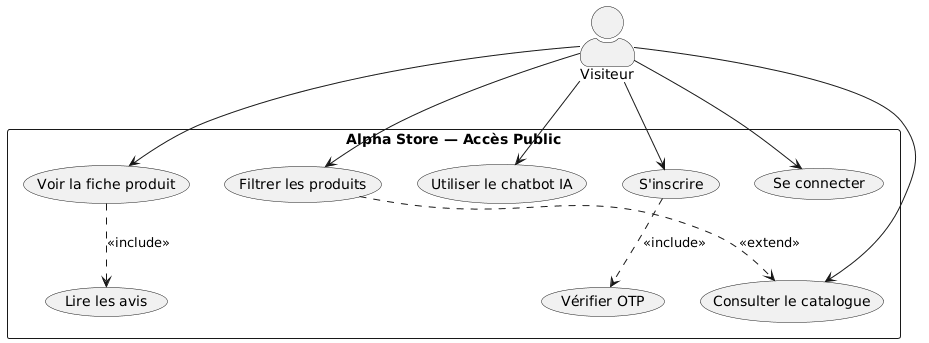
\includegraphics[width=0.7\textwidth]{chapitre2/figuresChap2/Visiteur.png}
    \caption{Diagramme de cas d'utilisation - Acteur Visiteur}
    \label{fig:uc_visiteur}
\end{figure}

\paragraph{Diagramme Utilisateur Connecté (Client) :} 
L'utilisateur connecté a accès aux fonctionnalités transactionnelles (panier, commande), sociales (avis, favoris) et aux outils d'intelligence artificielle avancés.
\begin{figure}[H]
    \centering
    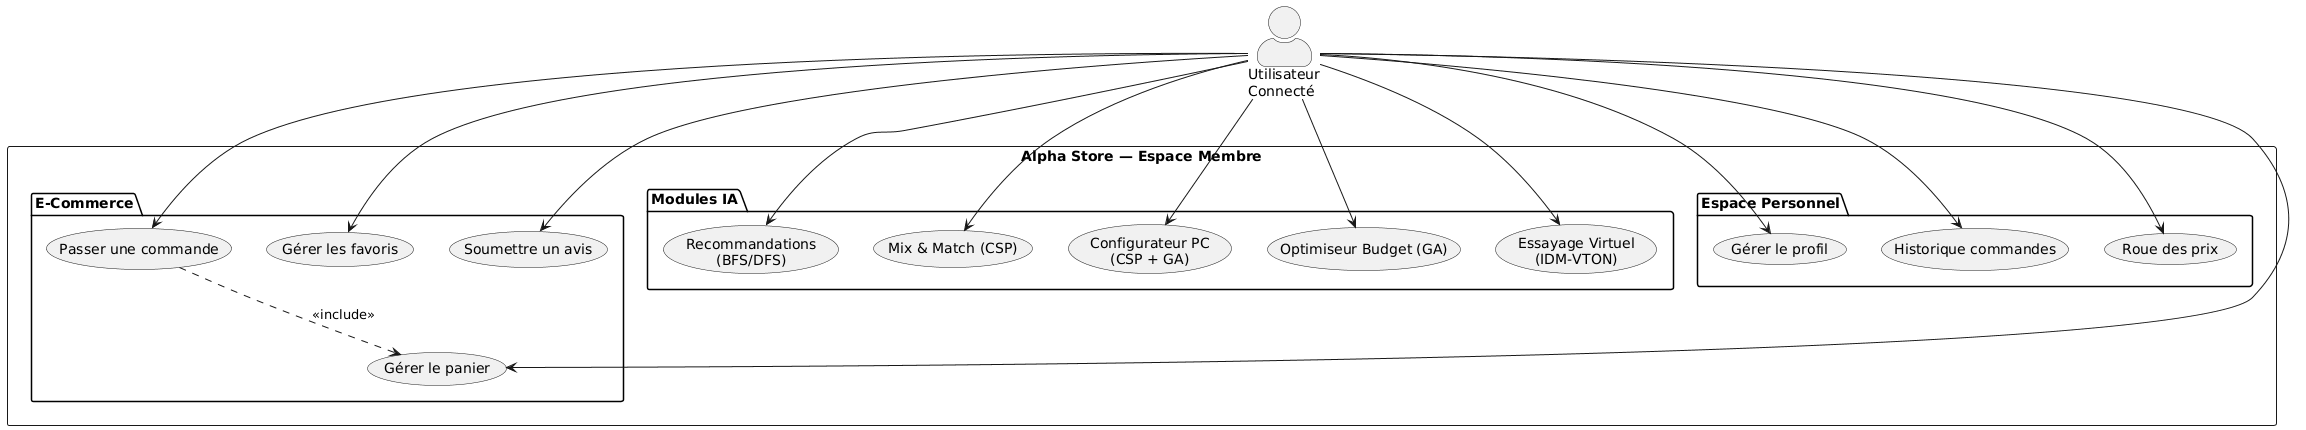
\includegraphics[width=0.8\textwidth]{chapitre2/figuresChap2/UtilisateurConnecté.png}
    \caption{Diagramme de cas d'utilisation - Acteur Client}
    \label{fig:uc_client}
\end{figure}

\paragraph{Diagramme Administrateur :} 
L'administrateur dispose de privilèges pour la gestion des stocks, des utilisateurs et le suivi global des activités.
\begin{figure}[H]
    \centering
    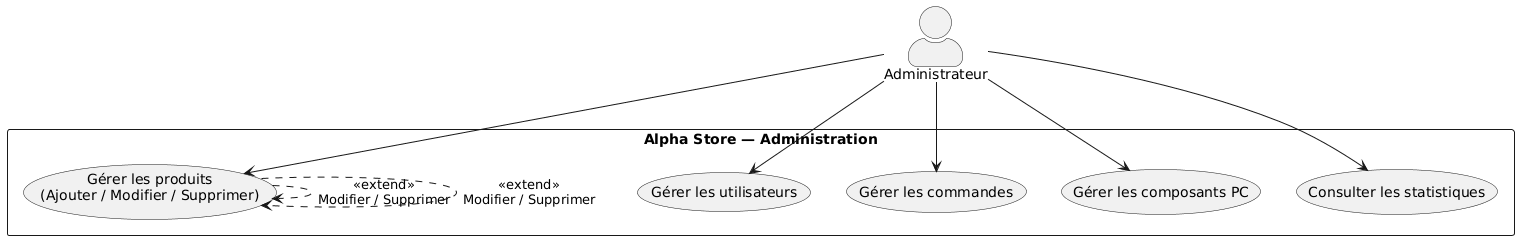
\includegraphics[width=0.7\textwidth]{chapitre2/figuresChap2/admin.png}
    \caption{Diagramme de cas d'utilisation - Acteur Administrateur}
    \label{fig:uc_admin}
\end{figure}

\subsection{Raffinement des cas d’utilisation}

\subsubsection{Analyse de cas d'utilisation : << Passer une commande >>}

Le diagramme ci-dessous (Figure \ref{fig:passe_commande}) détaille les étapes et les extensions possibles lors du processus de commande.

\begin{figure}[H]
    \centering
    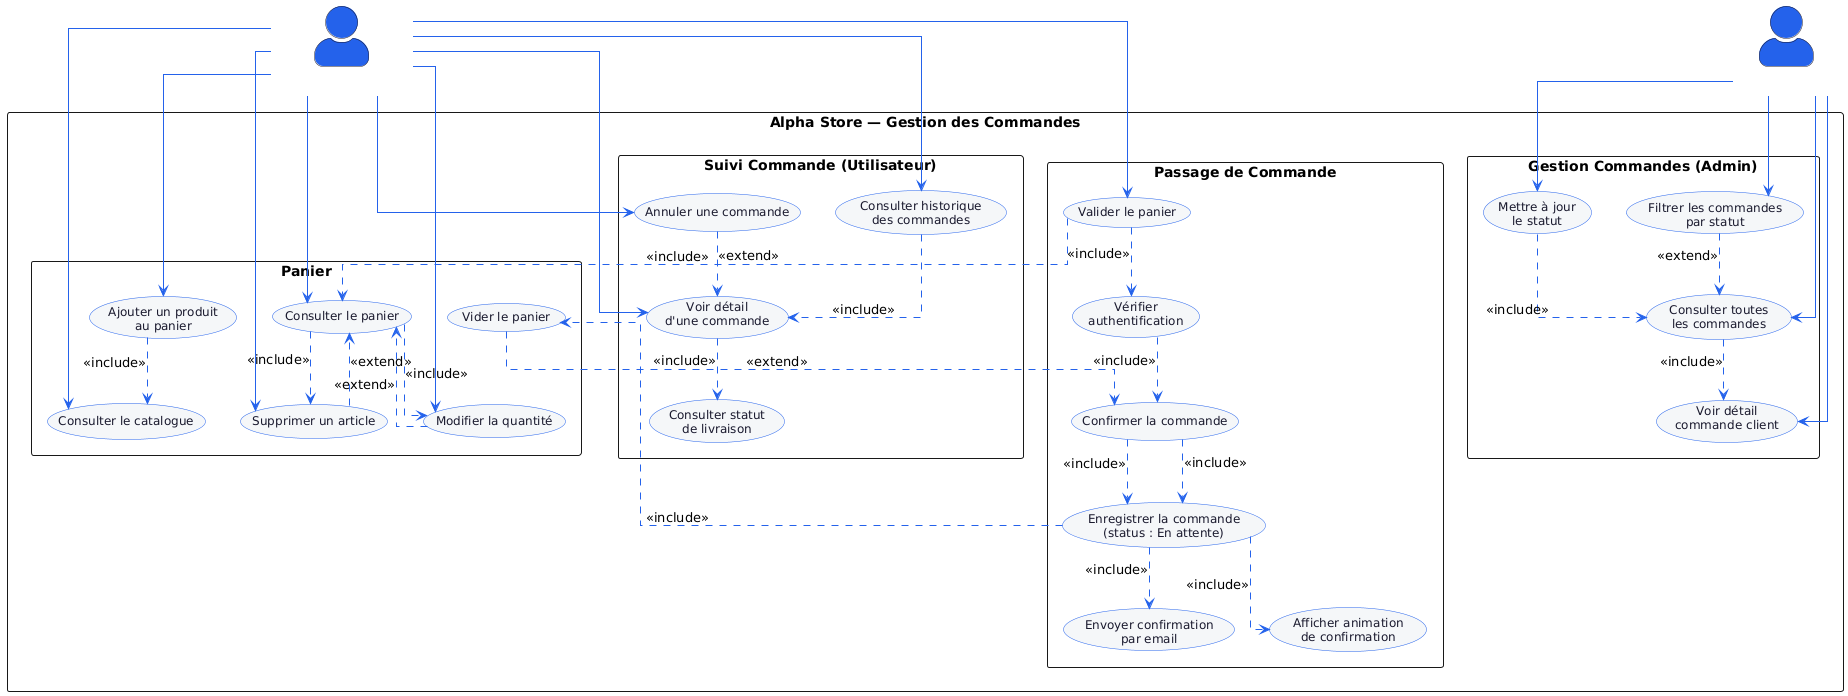
\includegraphics[width=0.9\textwidth]{chapitre2/figuresChap2/passecommande.png}
    \caption{Détail du cas d'utilisation << Passer une commande >>}
    \label{fig:passe_commande}
\end{figure}


\begin{table}[H]
\caption{Description textuelle du cas d’utilisation <<Passer une commande>>}
\begin{tabularx}{\textwidth}{|l|X|}
\hline
\textbf{Cas d'utilisation} & Passer une commande \\ \hline
\textbf{Acteur principal} & Client \\ \hline
\textbf{Pré-conditions} & Client connecté, panier non vide \\ \hline
\textbf{Scénario nominal} & 1. Le client valide son panier. 2. Le système vérifie le stock. 3. Le client confirme l'adresse. 4. Le système enregistre la commande. \\ \hline
\textbf{Post-conditions} & Commande enregistrée, stock mis à jour, email de confirmation envoyé. \\ \hline
\end{tabularx}
\label{tab:uc_commande}
\end{table}

\subsubsection{Analyse de cas d'utilisation : << Utiliser le Configurateur PC IA >>}

\begin{figure}[H]
    \centering
    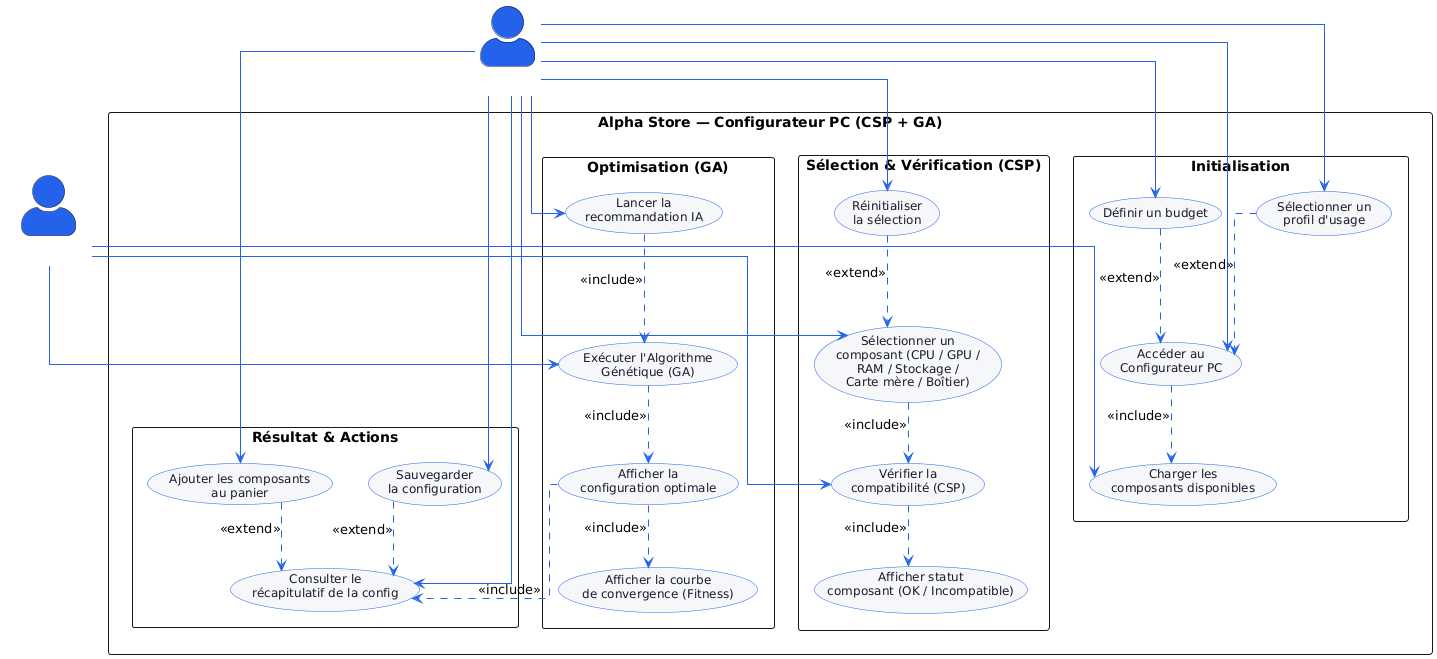
\includegraphics[width=0.85\textwidth]{chapitre2/figuresChap2/onfigurateurPC.png}
    \caption{Détail du cas d'utilisation << Configurateur PC IA >>}
    \label{fig:uc_pc_config}
\end{figure}

\begin{table}[H]
\caption{Description textuelle du cas d’utilisation <<Configurateur PC IA>>}
\begin{tabularx}{\textwidth}{|l|X|}
\hline
\textbf{Cas d'utilisation} & Configuration intelligente de PC \\ \hline
\textbf{Acteur principal} & Client \\ \hline
\textbf{Description} & Permet de générer une configuration PC compatible et optimisée selon un budget. \\ \hline
\textbf{Scénario nominal} & 1. Le client saisit son budget et son profil d'utilisation. 2. Le moteur CSP filtre les pièces compatibles. 3. L'algorithme génétique propose la meilleure combinaison. 4. Le client ajoute la configuration au panier. \\ \hline
\end{tabularx}
\label{tab:uc_pc_builder}
\end{table}

\section{Maquettes des interfaces (UI/UX)}

\subsection{Maquette : Page d'accueil dynamique}
La figure \ref{fig:maquette_homepage} présente la maquette de la page d'accueil d'Alpha Store. Elle met en évidence une interface moderne, épurée et interactive, conçue avec un slider dynamique animé via la bibliothèque GSAP. Cette page sert de point d'entrée unique et attractif pour diriger les utilisateurs vers les différents univers de la plateforme.

\begin{figure}[H]
    \centering
    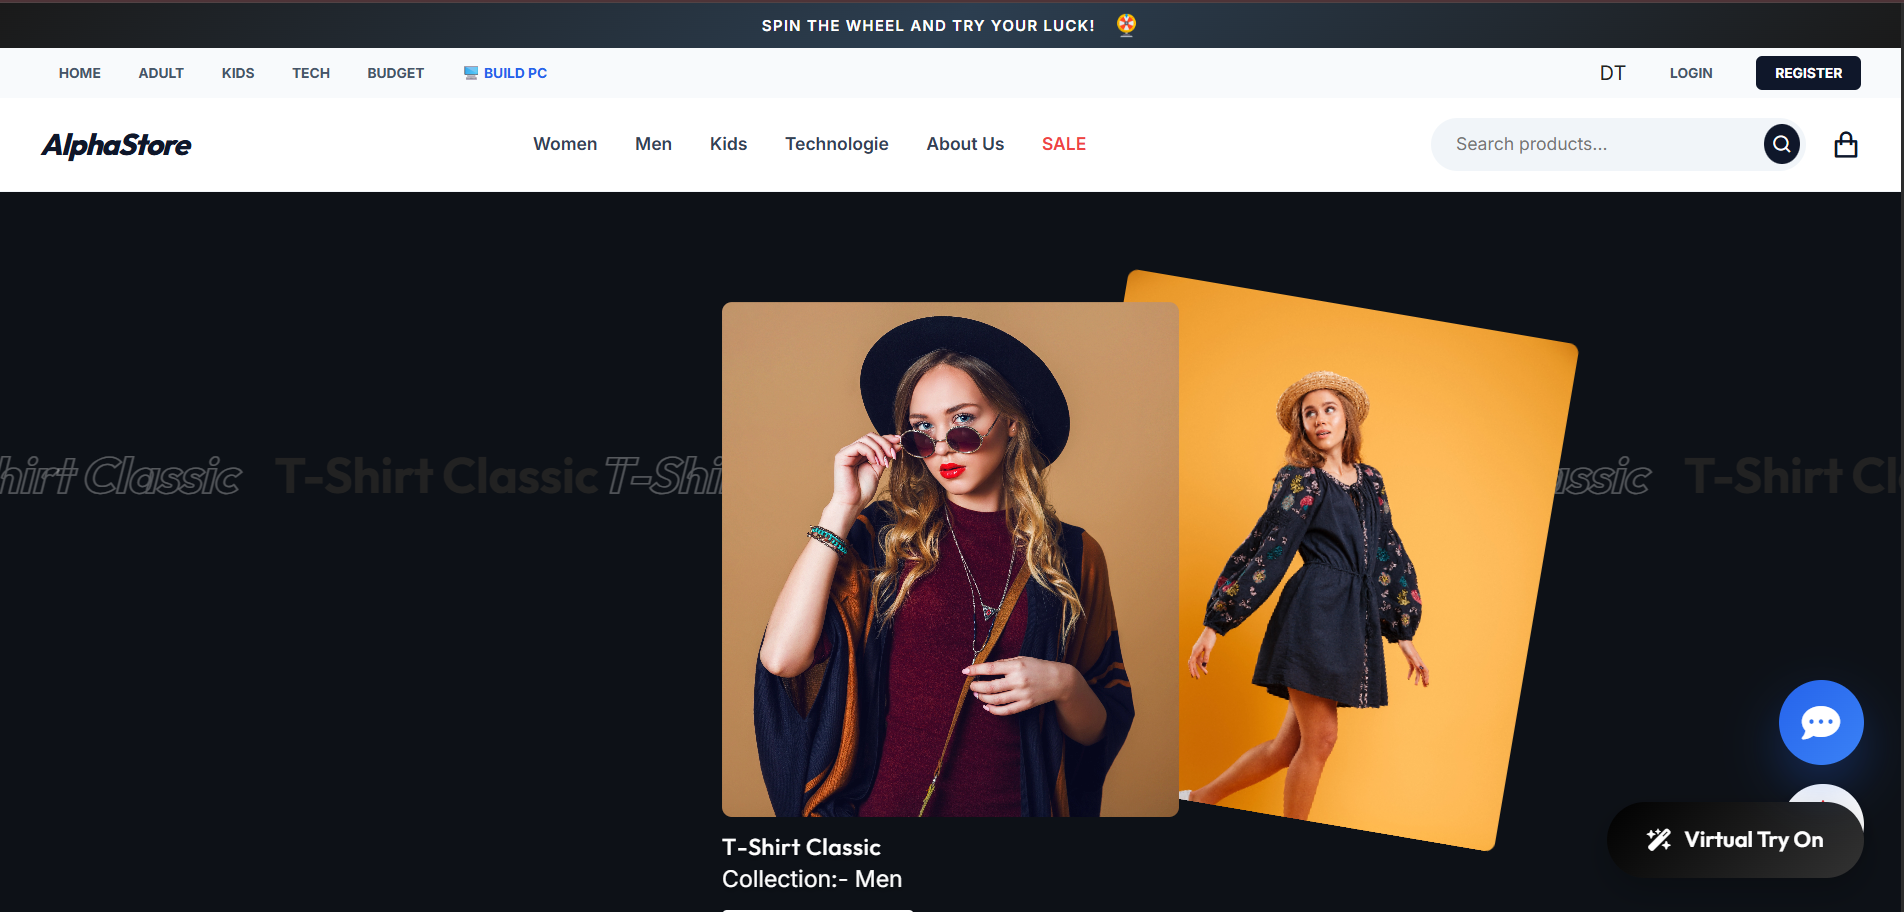
\includegraphics[width=0.95\textwidth]{chapitre2/maquettes/homepage.png}
    \caption{Maquette de la Page d'accueil dynamique}
    \label{fig:maquette_homepage}
\end{figure}

\subsection{Maquette : Système de gamification (Roue des prix)}
La figure \ref{fig:maquette_wheel} illustre la maquette du système de gamification, matérialisé par la << Roue de la fortune >> (Roue des prix). Cette fonctionnalité interactive vise à stimuler l'engagement et la fidélisation des utilisateurs en leur offrant la possibilité de remporter des récompenses exclusives, des remises ou des cadeaux directement sur la plateforme.

\begin{figure}[H]
    \centering
    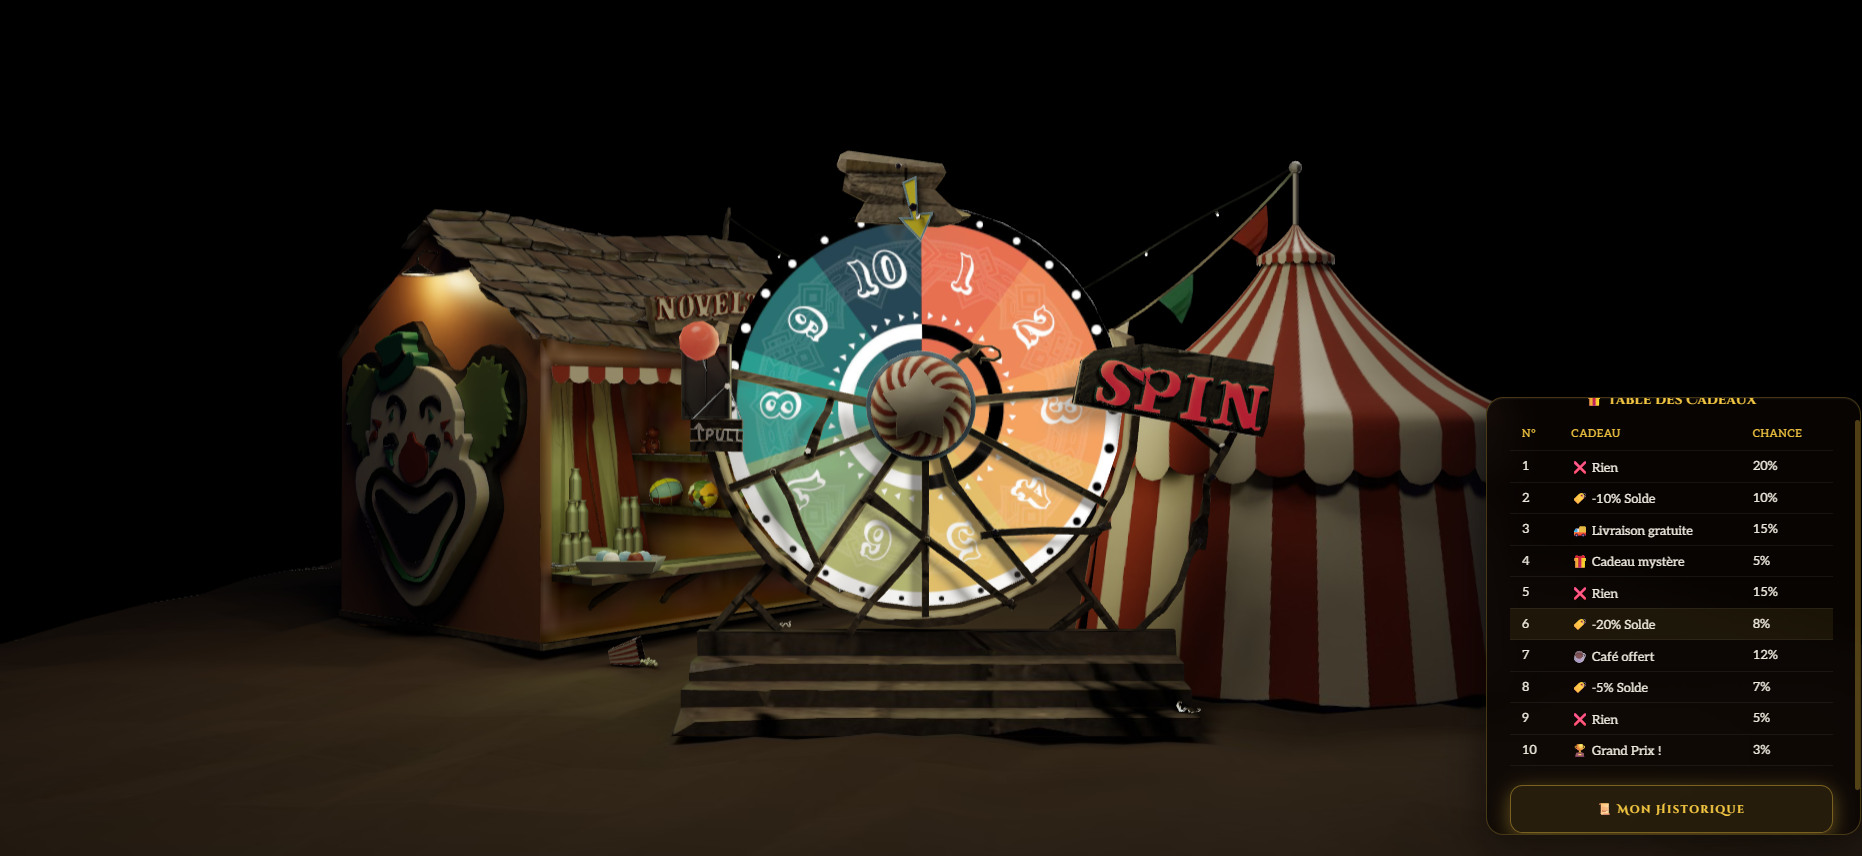
\includegraphics[width=0.95\textwidth]{chapitre2/maquettes/wheel_of_fortune.png}
    \caption{Maquette du Système de gamification (Roue des prix)}
    \label{fig:maquette_wheel}
\end{figure}

\subsection{Maquette : Hub d'Intelligence Artificielle}
La figure \ref{fig:maquette_hub_ia} représente le Hub d'Intelligence Artificielle, qui regroupe l'ensemble des outils intelligents développés pour accompagner l'utilisateur dans son parcours d'achat personnalisé. Cet espace centralise les modules tels que le Configurateur PC IA, le Mix \& Match, le Smart Budget et le Virtual Try-On.

\begin{figure}[H]
    \centering
    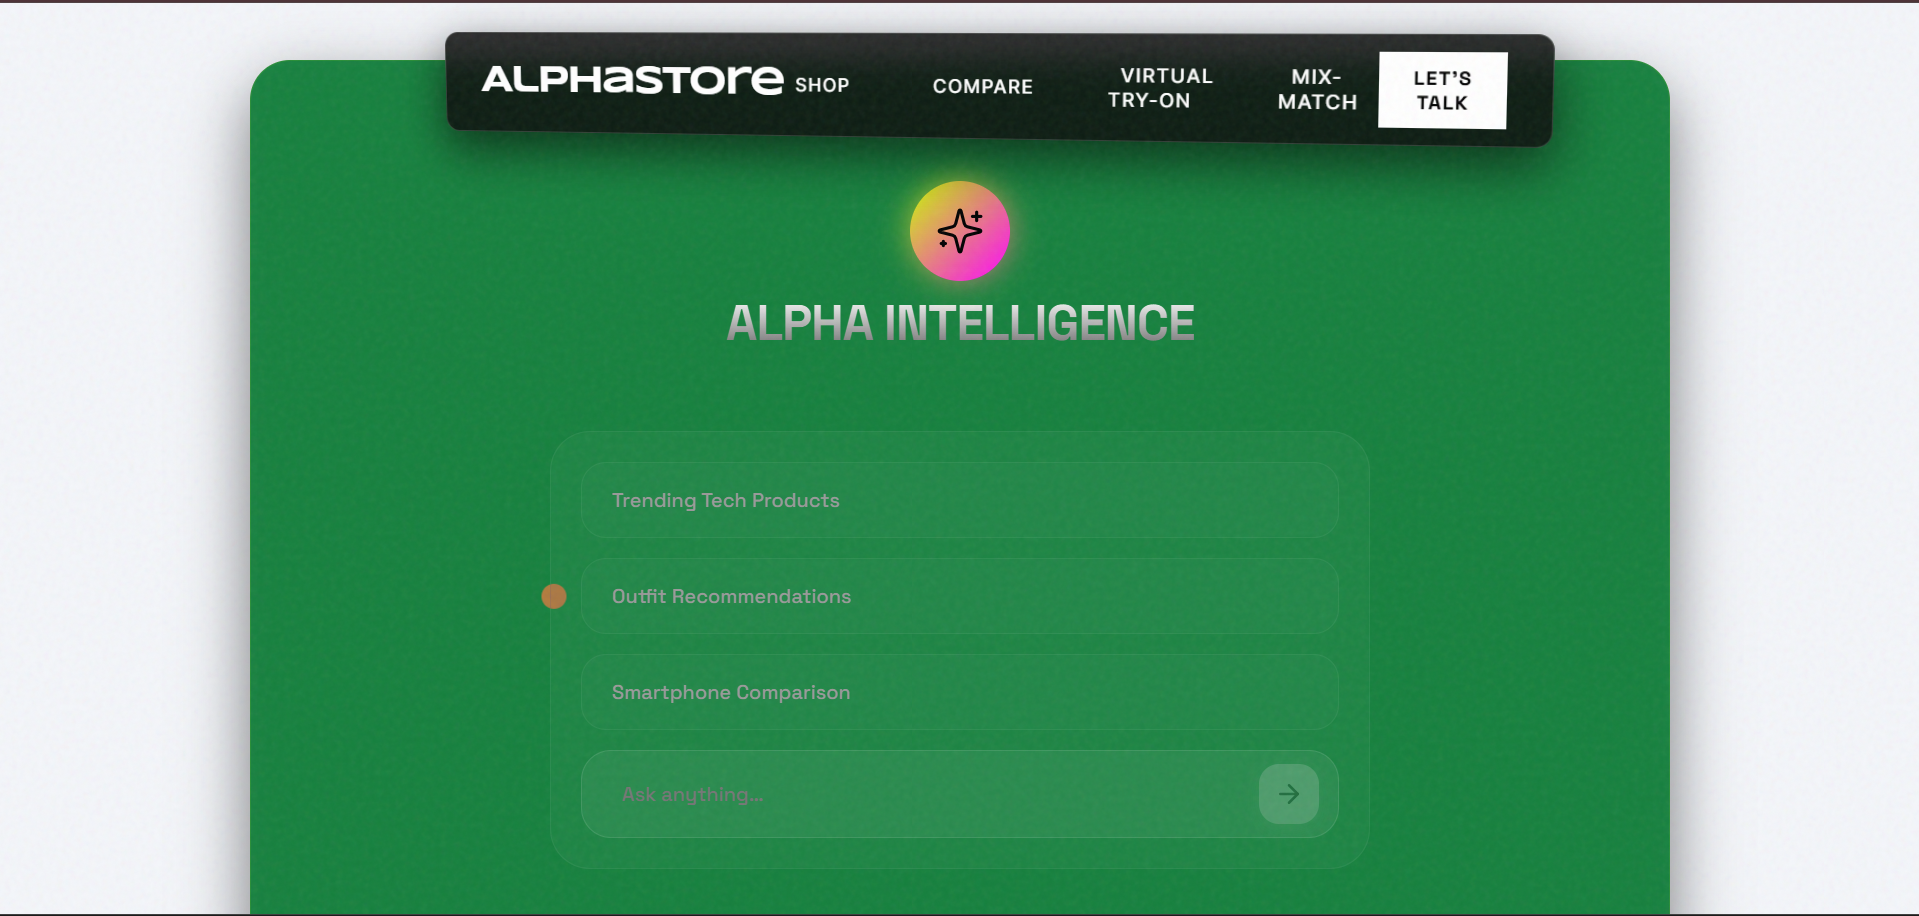
\includegraphics[width=0.95\textwidth]{chapitre2/maquettes/hub_ia.png}
    \caption{Maquette du Hub d'Intelligence Artificielle}
    \label{fig:maquette_hub_ia}
\end{figure}

\subsection{Maquette : Tableau de bord utilisateur}
La figure \ref{fig:maquette_dashboard_user} dévoile la maquette du tableau de bord utilisateur (dashboard client). Cet espace personnalisé permet au client de suivre ses commandes en temps réel, de gérer son profil et ses informations de livraison, de consulter son historique d'achats, et d'accéder rapidement à ses configurations sauvegardées.

\begin{figure}[H]
    \centering
    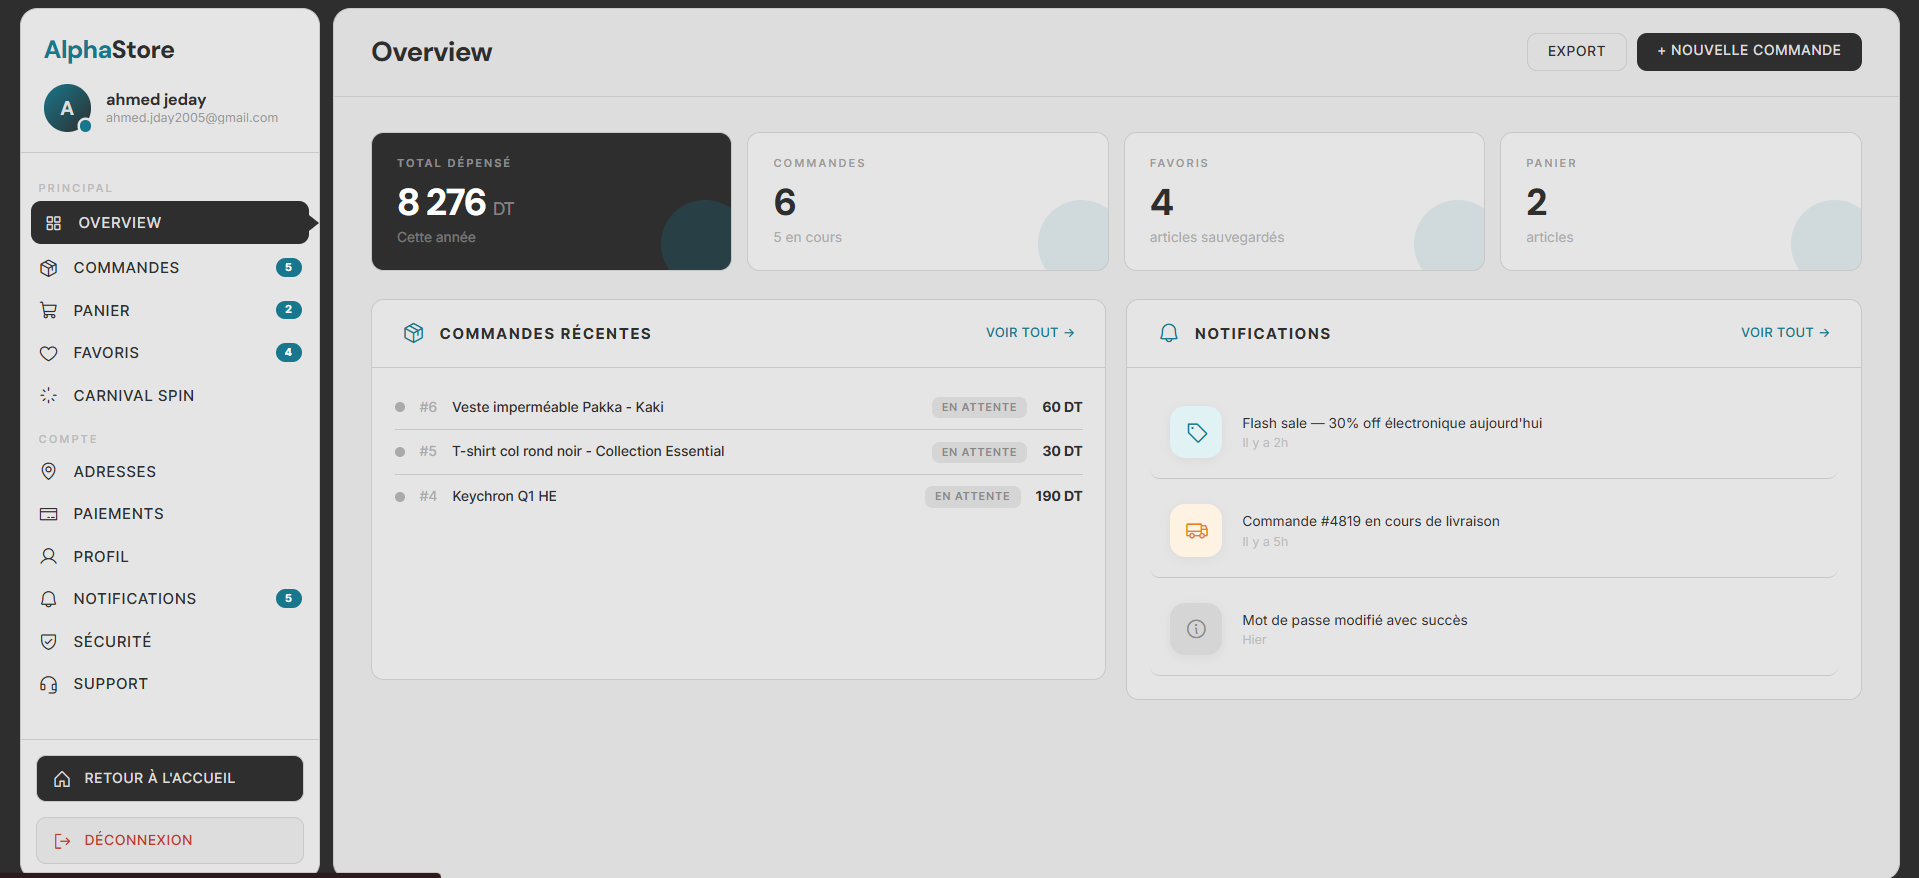
\includegraphics[width=0.95\textwidth]{chapitre2/maquettes/dashboard_user.png}
    \caption{Maquette du Tableau de bord utilisateur}
    \label{fig:maquette_dashboard_user}
\end{figure}

\section{Conclusion}

Ce chapitre a permis d'identifier et de structurer les attentes vis-à-vis de la plateforme Alpha Store. En définissant clairement les acteurs et les fonctionnalités, nous avons posé les jalons pour la phase de conception technique. L'intégration de l'intelligence artificielle au cœur des besoins fonctionnels distingue ce projet d'une solution e-commerce classique. Le chapitre suivant portera sur la conception architecturale et technique du système.
